\documentclass[11pt]{article}

\usepackage[margin=1in, headsep=5mm]{geometry}
\usepackage{amsmath}
\usepackage{graphicx}
\usepackage{enumerate}
\usepackage{fancyhdr}
\usepackage{hyperref}
\usepackage{authblk}

\parindent=\\
\linespread{1}


\newcommand{\units}[1]{\,\textrm{#1}}


%% This is a quick and dirty solution for multiple authors using the `authblk' package that comes with TeXlive
%% For a real journal article, you'll have to install the style packages used by that journal.
\title{Towards an Understanding of Below Breakdown Streamer Discharges Triggered With the Photoelectric Effect: Electrohydrodynamic Simulations of Pre-breakdown Electrons}

\author{Liam Keeley}
\affil{Department of Physics, Colorado College, Colorado Springs, CO 80903}%

\date{\today}% It is always \today
             %  but any date may be explicitly specified


\begin{document}

\pagestyle{fancy}
\lhead{\large Final Report}
\rhead{Liam Keeley}
%Next time: 
%  Move 1(c) to before 1(b)


\maketitle
\section{Introduction}
Streamer discharges

\section{Background}
If we imagine a single electron in a gas of otherwise neutral molecules, and we apply an electric field to this configuration, then the electron will be accelerated by the field, collide with molecules and lose momentum, and then be accelerated by the field again. In some cases, the electron will travel far enough between collisions that it has kinetic energy greater than the ionization energy of the molecule: then the electron can ionize that molecule. After such a collision, there will be two free electrons in the gas which can each ionize more molecules, but the collisions also result in ions which the electrons can reattach to. If the ionization rate is higher than the recombination rate, than a plasma known as a streamer will grow; otherwise, the streamer will be quenched. Because the ionization and recombination rates are related to the applied electric field, there is a specific electric field magnitude above which a streamer discharge will grow from one seed electron and below which it will not. This electric field is called the breakdown field. \\

When we consider many seed electrons, then streamer formation is more complicated. In some cases, the presence of many seed electrons can cause a streamer discharge even when the applied electric field is below breakdown. For example, Sun et al. \cite{Sun_2014} used a Particle In Cell simulation to show that a discharge can occur below breakdown in the presence of a high density parcel of seed ionization. Because this parcel has many free charges, it acts as an ideal conductor: the charges will position themselves to screen the applied field inside the parcel of ionized gas. This redistribution of charge results in the field being enhanced at the parcel's edges: in Sun et al.'s simulation, a streamer grew from the point where the field was locally above breakdown even when the applied field was below breakdown. \\

For my thesis, I will study another system in which I expect streamers to form below the breakdown field. Rather than a seed ionization, I will consider an external electron source. For concreteness, we could consider shining ultraviolet light onto the cathode of a parallel plate capacitor: the parallel plate capacitor provides the electric field and the ultraviolet light provides an external source of electrons from photo-emission. I expect the external source of electrons to form a cloud which will reinforce the applied electric field; similar to Sun et al.'s results, a streamer could grow from points where the local field exceeds the breakdown field. However, rather than simulating the streamer discharge, I only take the first step of demonstrating that conditions suitable for streamer formation can be achieved in this regime. To achieve this, I model the electron dynamics using electro-hydrodynamics. 


\section{Computer Simulation of Prebreakdown Electron Dynamics}
To study the behavior of released electrons prior to breakdown, I use fluid electro-hydrodynamics in 2D axis-symmetric coordinates. In this regime, it is assumed that enough electrons are released so that fluid models can be used and the random motion of individual electrons is insignificant. I assume that forces due to magnetic fields and pressure differentials are insignificant; prior to breakdown, there is no reason that either of these forces would be comparable to the applied electrostatic force. In fact, even after breakdown magnetic forces are generally insignificant \cite{Nijdam}. Finally, I assume axis-symmetry so that the electron density, electron drift velocity, and electric potential functions are all symmetric about an axis running through the center of each electrode. Thus, the inherently 3D process can be modelled in 2D rz-coordinates, significantly decreasing the computational difficulty of the problem. \\

With these assumptions in mind, describing the electron dynamics reduces to solving the following coupled partial differential equations. First, Poisson's Equation of electrostatics is used to resolve the electric potential everywhere given the electron density function. Then, once the electric potential is resolved, the electron fluid equation is used to describe the electron drift velocity. Finally, the electron continuity equation is used to update the electron density. By iteretively solving these three equations using finite difference methods, we can move our simulation forward in time and explore whether conditions for below breakdown streamer discharges can be achieved. 


\subsection{Poisson's Equation}
Poisson's equation follows from two of Maxwell's equations, Gauss's Law and Faraday's Law:
\begin{align}
    \nabla \cdot \vec{E} & = \frac{\rho}{\varepsilon_0} \\
    \nabla \times \vec{E} & = -\frac{\partial{\vec{B}}}{\partial{t}}
\end{align}

Where $\varepsilon_0$ is the permittivity of free space, $\rho$ is the charge density, $\vec{E}$ is the electric field, and $\vec{B}$ is the magnetic field. If we assume that $\frac{\partial{\vec{B}}}{\partial{t}} = 0$, then $\nabla \times \vec{E} = 0$ and we can write $\vec{E}$ as the gradient of a scalar potential $V$, $E=\nabla V$. Combining this with Gauss's Law, we arrive at Poisson's equation:

\begin{align}
    \nabla^2 V & = \frac{\rho}{\varepsilon_0} \text{, or in terms of the electron number density $n_e$:} \\
    \nabla^2 V & = -\frac{e}{\varepsilon_0}n_e
\end{align}

Which, when solved, gives the electric potential everywhere in space and can be used to determine the electric force felt by the electrons.

\subsection{Continuity Equation and Electron Fluid Equation}
The electron fluid equation is often derived in plasma physics from the Vlasov equation, which is a continuity equation in phase space. To emphasize the similarities between these two equations, I will begin by deriving the continuity equation from conservation of electron number, and then I will give a derivation of Vlasov's equation; from Vlasov's equation, I will re-derive the continuity equation, then derive the electron fluid equation. Finally, I will derive the fluid equation directly from Newton's Second Law. \\

The continuity equation is fundamentally a statement about any quantity which is locally conserved: in our specific case, it is the electron number density which is conserved. Consider a volume $V$ in which the electron number density is $n_e=n_e(t,x,y,z)$: the total number of electrons in this volume is:

\begin{equation}
    N = \int_{V} n_e dV
\end{equation}

The rate of change of $N$ in our volume is then:

\begin{align}
    \frac{dN}{dt} & = \frac{d}{dt}\int_{V}n_e dV, \text{ and by the Leibniz Integral Rule:} \\
    & = \int_{V}\frac{\partial{n_e}}{\partial{t}}dV
\end{align}

Now comes the important step: we assume local conservation of electron number so that no electrons are created or destroyed inside our volume. Then, the number of electrons inside the volume can only change if electrons pass across the boundary of the volume. If we define the electron drift velocity $\vec{u}_e=\vec{u}_e(x,y,z)$ to be the average velocity of electrons at each point space, then the rate at which electrons cross the boundary is:

\begin{equation}
    \frac{dN}{dt} = -\oint_{\partial V}{(n_e\vec{u}_e)\cdot d\vec{A}}
\end{equation}

Where $\partial V$ is the boundary of our volume. Because electrons are not created or destroyed inside the volume, this is the rate of change of the number of electrons inside the volume as well, and so:

\begin{align}
    \int_V{\frac{\partial n_e}{\partial t}}dV &= -\oint_{\partial V} (n_e\vec{u}_e)\cdot d\vec{A} \\
    \int_V{\frac{\partial n_e}{\partial t}}dV + \oint_{\partial V} (n_e\vec{u}_e)\cdot d\vec{A} &= 0 \\
    \int_V{\frac{\partial n_e}{\partial t} + \nabla \cdot (n_e \vec{u}_e) dV} & = 0
\end{align}

Where the Divergence Theorem was used in the last step. This integral must be satisfied for any volume in which electron number is locally conserved, which we assume to be everywhere in our domain. Thus, if the integral statement were satisfied but the integrand $\frac{\partial{n_e}}{\partial t} + \nabla \cdot (n_e \vec{u}_e)$ were not $0$ somewhere in the volume, then the integrand would also have to be nonzero at least one other place in the volume so that the total integral were still $0$. Because we took $V$ to be arbitrary, we can define a new volume around one of these points in which the integral would be nonzero, contradicting our assumption of local electron number conservation. Therefore, we conclude the continuity equation:

\begin{equation}
    \frac{\partial{n_e}}{\partial t} + \nabla \cdot (n_e \vec{u}_e) = 0
\end{equation}

Must be true everywhere that electron number density is locally conserved. We can write this in terms of generalized spacial coordinates $\{x_1,x_2,x_3\}$ as:

\begin{equation}
    \partial_t{n} + \partial_i{(n u_i)} = 0
\end{equation}

Where it is understood that $\partial_t = \frac{\partial}{\partial t}$, $\partial_i = \frac{\partial}{\partial x_i}$, and repeated indices are summed over. This notation highlights the generality of the continuity equation: it applies to any space in which a quantity is locally conserved. 

\subsection{Phase Space}

Next, we derive the Vlasov equation, which is an equation of continuity in phase space. Phase space is a six dimensional vector space where a particle's coordinates are described by the three spacial coordinates $(x,y,z)$ as well as three velocity coordinates $(v_x,v_y,v_z)$. Thus, for two particles to have the same position in phase space, they must not only have the same position in physical space, but must also be moving with the exact same velocity. In analogy to a number density function $n_e=n_e(t,x,y,z)$ in physical space, we can define a function $\Tilde{n}_e=\Tilde{n}_e(t,x,y,z,v_x,v_y,v_z)$ in phase space. Similarly, we have a volume element $d\Tilde{V} = dxdydzdv_xdv_ydv_z$, and the number of particles in a phase space volume $\Tilde{V}$ is:

\begin{equation}
    \Tilde{N} = \int_{\Tilde{V}} \Tilde{n}_e d\Tilde{V}
\end{equation}

So:

\begin{equation}
    \frac{d\Tilde{N}}{dt} = \frac{d}{dt}\int_{\Tilde{V}} \Tilde{n}_e d\Tilde{V} = \int_{\Tilde{V}}\frac{\partial \Tilde{V}}{\partial t} d\Tilde{V}
\end{equation}

Again, we assume local conservation of electron number in phase space. The flux element at each point on the surface can again be defined as $n_e\vec{u}_e$, but we need to think carefully about what the components of $\vec{u}_e$ are. If we consider a surface oriented in the $\hat{x}$ direction, then the rate at which electrons pass through each point on the surface is $n_e\frac{dx}{dt}=n_ev_x$. In the case of the continuity equation, we used the average velocity; however, the velocity is precisely defined at each point in phase space, so this is unnecessary for Vlasov's equation. If the surface is oriented in the $\hat{v_x}$ direction, then the rate at which electrons pass through each point on the surface is $n_e\frac{dv}{dx}=n_ea_x$, where $a_x$ is the acceleration of the particle. Note that the acceleration is not exactly defined at each point in phase space like the velocity is: this acceleration is the average acceleration across the boundary. Regardless, we define $\mathbf{\tilde{u}}_e=(v_x,v_y,v_z,a_x,a_y,a_z)$, and the number of electrons crossing the boundary is:

\begin{equation}
    \frac{d\Tilde{N}}{dt} = -\oint_{\Tilde{S}}{(\Tilde{n}_e \mathbf{\Tilde{u}}_e) \cdot d \mathbf{\Tilde{A}}} = -\int_{\Tilde{V}} \Tilde{\nabla} \cdot (\tilde{n}_e \mathbf{\Tilde{u}_e}) d\Tilde{V}
\end{equation}

Where $\Tilde{\nabla} = (\frac{\partial}{\partial x},\frac{\partial}{\partial y},\frac{\partial}{\partial z},\frac{\partial}{\partial v_x},\frac{\partial}{\partial v_y},\frac{\partial}{\partial v_z})$. Again, because electron number is locally conserved:

\begin{equation}
    \int_{\Tilde{V}}\frac{\partial \Tilde{n}_e}{\partial t} d\Tilde{V} + \int_{\Tilde{V}} \Tilde{\nabla} \cdot (\tilde{n}_e \mathbf{\Tilde{u}_e}) d\Tilde{V} = 0
\end{equation}

And because this applies for all phase space volumes:

\begin{equation}
    \frac{\partial \Tilde{n}_e}{\partial t} + \Tilde{\nabla} \cdot (\tilde{n}_e \mathbf{\Tilde{u}_e}) = 0
\end{equation}

Which is the Vlasov Equation. We can write this in the regular way by defining $\nabla'=(\frac{\partial}{\partial v_x}, \frac{\partial}{\partial v_y}, \frac{\partial}{\partial v_z})$ and expanding $\Tilde{\nabla}$ in terms of $\nabla$ and $\nabla'$:

\begin{equation}
    \frac{\partial \Tilde{n}_e}{\partial t} + \nabla \cdot (\Tilde{n}_e \vec{v}) + \nabla' \cdot (\Tilde{n_e}\vec{a}) = 0
\end{equation}




\section{Results}

\begin{figure}
    \centering
    \includegraphics{Example_Boosted_V.pdf}
    \caption{An example of what I want the electric field to look like as a function of time (this is from a somewhat unrealistic run)}
    \label{fig:boosted}
\end{figure}

\begin{figure}
    \centering
    \includegraphics[scale=0.6]{Example_Evolution_Fig.pdf}
    \caption{Example electron density evolution figure. Again, not a super realistic example}
    \label{fig:evolution}
\end{figure}

\section{Works Cited}

\section{Appendix A: Finite Difference Equations}
\subsection{Poisson's Equation}
Where $e$ is the electron charge. To solve this computationally, we approximate it as the diffusion equation:

\begin{align}
    \frac{\partial{V}}{\partial{t}} = & \nabla^2 V - \frac{e}{\varepsilon_0} n_e \text{, or in cylindrical coordinates: } \\
    \frac{\partial{V}}{\partial{t}} & = \frac{\partial^2{V}}{\partial{z}^2} + \frac{1}{r}\frac{\partial}{\partial{r}}\left[ r \frac{\partial{V}}{\partial r}\right] - \frac{e}{\varepsilon_0}n_e
\end{align}

Which becomes exact as $t \to \infty$ and $\frac{\partial{V}}{\partial{t}} \to 0$. Because we have no spatial first derivatives in this equation, a forward difference scheme for the time derivative and centered derivatives for the spatial derivatives will be stable \cite{numerical}, giving the following scheme:

\begin{multline}
    \frac{V^{n+1}_{j,l}-V^{n}_{j,l}}{\Delta t} = \frac{1}{\Delta z}\left[ V^n_{j+1,l} - 2V^{n}_{j,l}+V^{n+1}_{j-1,l} \right] 
    \\ + \frac{1}{r_{j,l} \Delta r} \left[ \frac{r_{j,l+\frac{1}{2}} (V^n_{j,l+1} - V^n_{j,l}) - r_{j,l-\frac{1}{2}}*(V^n_{j,l} - V^n_{j,l-1})}{\Delta t} \right] - \frac{e}{\varepsilon_0}n^n_{j,l}
\end{multline}

We can then use the stability condition $\Delta t = \frac{\Delta r^2}{4} = \frac{\Delta z^2}{4}$ to end up with:

\begin{equation}
    4V^{n+1}_{j,l} = V^n_{j+1,l} + V^{n}_{j-1,l} + \frac{r_{j,l}+\frac{\Delta r}{2}}{r_{j,l}}V^n_{j,l+1} + \frac{r_{j,l} - \frac{\Delta r}{2}}{r_{j,l}} V^n_{j,l-1} - \frac{e}{\varepsilon_0}n^n_{j,l} \Delta r \Delta z
\end{equation}

For boundary conditions, we assume that the potential is positive at the cathode and zero at the anode as well as at large $r$. The boundary at $r=0$ is tricky due to the singularity which occurs here. To deal with it, we consider our original diffusion equation in the limit as $r \to 0$:

\begin{align}
    \frac{\partial{V}}{\partial{t}} &= \frac{\partial^2{V}}{\partial{z^2}} + \lim_{r\to0}\left[{\frac{1}{r}\frac{\partial}{\partial{r}} \left[ r \frac{\partial{V}}{\partial{r}}\right]}\right] - \frac{e}{\varepsilon_0}n_e \\
    &= \frac{\partial^2{V}}{\partial{z^2}} + \lim_{r\to0}\left[\frac{\partial^2{V}} {\partial{r^2}} + \frac{1}{r}\frac{\partial{V}}{\partial{r}}\right] - \frac{e}{\varepsilon_0}n_e \\
     &= \frac{\partial^2{V}}{\partial{z^2}} + 2\frac{\partial^2V}{\partial{r^2}} - \frac{e}{\varepsilon_0}n_e
\end{align}

Finite differencing this, we find that:

\begin{equation}
    \frac{V^{n+1}_{j,0}-V^{n}_{j,0}}{\Delta t} = \frac{1}{\Delta z^2}\left[ V^n_{j+1,0} - 2V^n_{j,l} + V^{n}_{j-1,0}\right] + \frac{2}{\Delta r} \left[ V^n_{j,1} - 2V^n_j,0 + V^n_{j,-1}\right] - \frac{e}{\varepsilon_0}n^n_{j,l}
\end{equation}
By symmetry, $V$ must be the same on each side of the $r=0$ boundary, so $V^n_{j,l} = V^n_{j,-l}$. Again using the stability condition $\Delta t = \frac{\Delta r^2}{4} = \frac{\Delta z^2}{4}$, we find that:

\begin{equation}
    4V^{n+1}_{j,0} = 2V^{n}_{j,0} + 4V^n_{j,1} + V^n_{j+1,0} + V^n_{j-1,0}-\frac{e}{\varepsilon_0}n^n_{j,0}\Delta r \Delta z
\end{equation}

And so we have described all boundaries and achieved a consistent scheme for our diffusion equation; we can then iteritevely solve this to relax to a steady state solution for $V$ and thus solve Poisson's Equation (specifically, we use successive over relaxation–see Chapter 20 of \cite{numerical} for details). \\

To verify this scheme, I compare the analytic solution of Poisson's Equation in cylindrical coordinates to the numerical solution in Figure \ref{fig:analytic_laplace}.

\begin{figure}
    \centering
    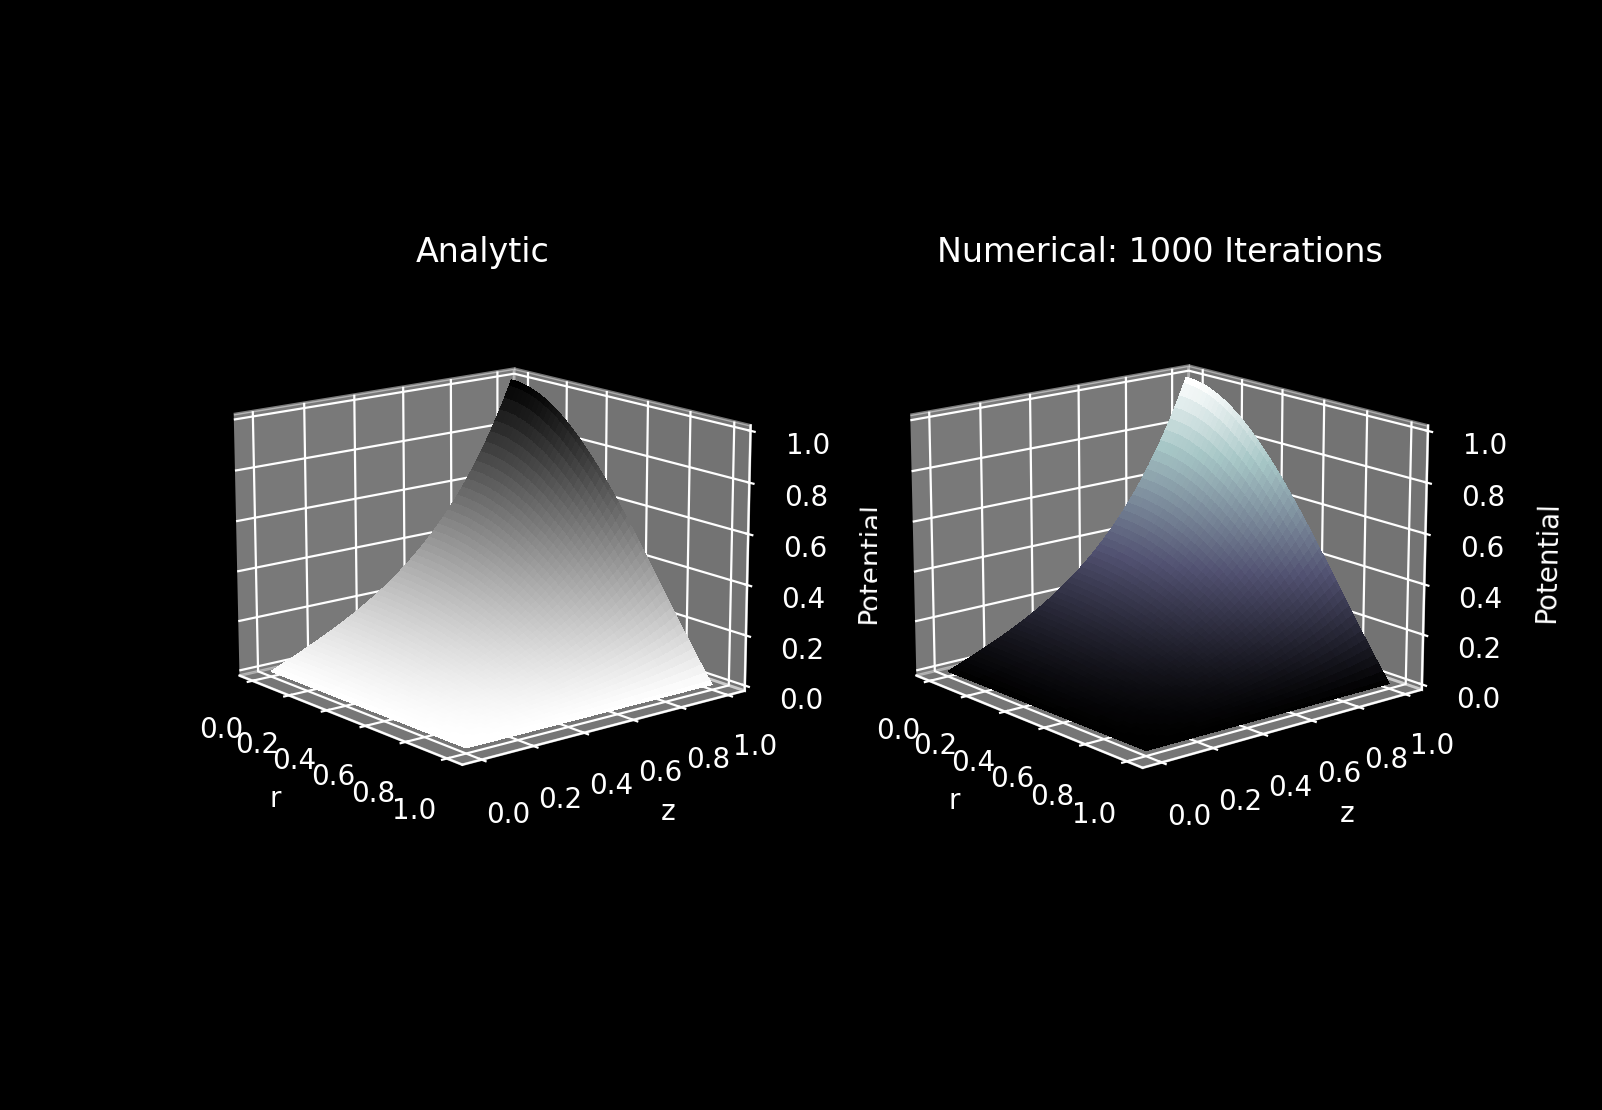
\includegraphics[scale=0.2]{rz_analytic_numerical.png}
    \caption{Comparison of the analytic solution to Laplace's Equation in rz-coordinates.}
    \label{fig:analytic_laplace}
\end{figure}

\subsection{Electron Fluid Equation}

\subsection{Electron Continuity Equation}
The continuity equation comes from the assumption that electron density cannot be created or destroyed spontaneously, and so material entering one point in space must be coming from another point in space. In axis-symmetric cylindrical coordinates, our finite volume elements are concentric disks. If we center these volumes on one of our computational grid points, then adjacent points will be on the face of this volume, and the electron flux across each face will be the product of the area of that face, the electron density at the face, and the normal component of the electron drift velocity at that face. The change in the electron density in this volume element is the total flux entering (or leaving) it divided by the volume of the element:

\begin{equation}
    \frac{\Delta n{j,l}}{\Delta t} = \frac{A_{j,l+1}u^n_{rj,l+1}n^n_{j,l+1}-A_{j,l-1}u^n_{rj,l-1}n^n_{j,l-1}}{V} + \frac{A_{j+1,l}u^n_{z j+1,l}n^n_{j+1,l}-A_{j-1,l}u^n_{zj-1,l}n^n_{j-1,l}}{V} 
\end{equation}

From geometry, we know our volume element is $V=2 \pi (r^2_{j,l+1}-r^2_{j,l-1}) \Delta z$, while our area elements are $A_{j,l+1} = 4 \pi r_{j,l+1} \Delta z$, $A_{j,l-1} = 4 \pi r_{j,l-1} \Delta z$, $A_{j+1,l}=A_{j-1,l}=\pi(r^2_{j,l+1}-r^2_{j,l-1})$. Then, using a time centered leapfrog scheme:

\begin{multline}
    \frac{ n^{n+1}_{j,l} - n^{n-1}_{j,l}}{2\Delta t} = \frac{2}{r^2_{j,l+1}-r^2_{j,l-1}} \left[ r_{j,l+1}u^n_{rj,l+1}n^n_{j,l+1}-r_{j,l-1}u^n_{rj,l-1}n^n_{j,l-1} \right] +  \frac{1}{2 \Delta z}\left[ u^n_{z j+1,l}n^n_{j+1,l}-u^n_{zj-1,l}n^n_{j-1,l} \right]
\end{multline}

\begin{multline}
    n^{n+1}_{j,l} = n^{n-1}_{j,l} + \frac{4\Delta t}{r^2_{j,l+1}-r^2_{j,l-1}}\left[ r_{j,l+1}u^n_{rj,l+1}n^n_{j,l+1}-r_{j,l-1}u^n_{rj,l-1}n^n_{j,l-1}\right] + \\
    \frac{\Delta t}{\Delta z} \left[ u^n_{z j+1,l}n^n_{j+1,l}-u^n_{zj-1,l}n^n_{j-1,l} \right]
\end{multline}

At the $r=0$ boundary, symmetry dictates that no net flux passes over the boundary. This leaves us with the following:

\begin{equation}
    n^{n+1}_{j,0} = n^{n-1}_{j,0} + \frac{4\Delta t}{r_{j,1}} u^n_{rj,1}n^n_{j,1} +
    \frac{\Delta t}{\Delta z} \left[ u^n_{z j+1,0}n^n_{j+1,0}-u^n_{zj-1,0}n^n_{j-1,0} \right]
\end{equation}

At the anode, we want electron density to be absorbed, and similarly, at large $r$, we want density to pass out of the computational domain, so we choose diffuse boundary conditions in which normal spacial derivatives vanish. In one dimension, the method for achieving this is to set the value equal to adjacent points \cite{computational}. What I have done here is to do this, but combine this with a step in the direction parallel to the surface, resulting in the following boundary conditions:

\begin{align}
n^{n+1}_{j,L} &= n^n_{j,L-1} - \frac{\Delta t}{\Delta z} \left[ n^n_{j+1,L}u^n_{z j+1, L}-n^n_{j-1,L}u^n_{z j-1,L} \right] \text{ (at $r_{max}$)} \\
n^{n+1}_{J,l} &= n^n_{J-1,l} - \frac{4 \Delta t}{r_{l+1}^2-r_{l-1}^2} \left[ r_{l+1}n^n_{J,l+1}u^n_{r J,l+1} - r_{l-1}n^n_{J,l-1}u^n_{r J,l-1}\right] \text{ (at $z_{max}$)}
\end{align}


\section{Appendix A: Analytic Solution to Laplace's Equation In rz-Coordinates}
In cylindrical rz-coordinates, Laplace's Equation is:

\begin{align}
    \nabla^2V & = 0 \\
    \frac{\partial^2V}{\partial z^2} + \frac{1}{r} \frac{\partial}{\partial r}\left[ r \frac{\partial V}{\partial r}\right] & = 0
\end{align}

We can solve this by separation of variables. We begin by guessing that $V(r,z)=R(r)Z(z)$. Then:

\begin{align}
    \frac{\partial^2\left[R(r)Z(z)\right]}{\partial z^2} + \frac{1}{r} \frac{\partial}{\partial r}\left[ r \frac{\partial \left[R(r)Z(z)\right]}{\partial r}\right] & = 0 \\
    R\frac{\partial^2 Z}{\partial z^2} + \frac{Z}{r} \frac{\partial}{\partial r} \left[ r\frac{\partial R}{r}\right] & = 0 \\
    \frac{1}{Z} \frac{\partial^2Z}{\partial z^2} & = -\frac{1}{rR}\frac{\partial}{\partial r} \left[ r \frac{\partial R}{\partial r}\right]
\end{align}

Because the left side of this equation has no $z$ dependence and the right side has no $r$ dependence, and this must hold for all $r,z$, it follows that this equality must be some constant $k$, so:

\begin{align}
    \frac{\partial^2Z}{\partial z^2} &= kZ, \text{ and:}\\
    \frac{\partial}{\partial r}\left[ r\frac{\partial R}{\partial r }\right] &= -krR \\
    \frac{r^2}{R} \frac{\partial^2R}{\partial r^2} + \frac{r}{R} \frac{\partial R}{\partial r} + kr^2 & = 0
\end{align}

If we take $k = \alpha^2 > 0$ – meaning that the solution is exponential in $z$ – 



\begin{thebibliography}{9}
\bibitem{Sun_2014}
Anbang Sun et al 2014 J. Phys. D: Appl. Phys. 47 445205

\bibitem{Nijdam}
Sander Nijdam et al., 2020. \textit{Plasma Sources Sci. Technol.} \textbf{29} 103001.

\bibitem{Bellan}
Bellan, Paul, \textit{Fundamentals of Plasma Physics}. Cambridge University Press, 2006. 

\bibitem{numerical}
William Press, Saul Teukosky, William Vetterling, and Brian Flannery, \textit{Numerical Recipes: The Art of Scientific Computing.} Cambridge University Press, 2007.


\bibitem{computational}
Franklin, Joel. \textit{Computational Methods For Physics}.

\bibitem{Neuenschwander}
Neuenschwander, Dwight. \textit{Emmy Noether's Wonderful Theorem}
\end{thebibliography}
\end{document}





\end{document}

